\chapter{When Hard Work Misses the Basics}

This chapter follows a short School of Hard Knocks interview segment, curated for this book by LazyingArt LLC through Video2Book. The interviewer asks what football taught that later mattered in business ownership and leadership. The answer first passes through the usual language of teamwork and adversity, then turns toward something more uncomfortable: the speaker's most useful lesson came from the way his own hard work was weakened by refusing the basics.

\section{The Question of Transfer}

The opening question is a transfer question. We are asked to follow a habit from one arena, football, into another arena, business leadership. That is the right scale for the chapter. The point is not that sports automatically produce good business owners. The point is that a particular experience can become useful when it exposes a repeatable discipline.

The speaker's answer begins in the familiar place. Football teaches a person to work with a team and to deal with adversity. Those lessons matter, but they do not yet explain the distinctive mechanism of this story. They are the entrance to the argument, not its conclusion.

\section{The Common Lessons}

Teamwork and adversity are the expected lessons because they are visible from the outside. Anyone watching a team sport can see cooperation, pressure, loss, fatigue, and recovery. The speaker grants that much, but he also marks those lessons as common.

That transition is important. If we stop at teamwork and adversity, the chapter becomes a generic slogan about sports and character. The speaker is doing something narrower. He is asking us to look at the mistake that made the lesson stick.

\begin{remark}
The common lessons should remain in the notes because they set the baseline. But the useful entrepreneurial payload begins only when the speaker turns from general sports virtues to the specific failure in his own learning.
\end{remark}

\section{The Lesson Came From Mistakes}

The pivot is direct: the best lesson came from mistakes in sports. That changes the tone of the answer. A success story usually invites imitation. A mistake invites diagnosis.

Here the mistake is not laziness. It is not lack of ambition. It is not the absence of strong teachers. The mistake is more subtle: he had effort, and he had coaching, but he did not let the coaching govern the work deeply enough. In business terms, this is the difference between intensity and disciplined improvement.

\section{Quarterback, College, and Coaches}

The speaker then gives the setting. He played quarterback, and he describes himself as a scrappy dual-threat quarterback. That role matters because a quarterback is not merely an athlete executing isolated tasks. A quarterback has to read, decide, coordinate, and still operate inside a structure. The role makes the later lesson about basics more concrete.

The setting is Long Beach City College, a junior college just outside Los Angeles. He names Brad Peabody and Ryan Flynn as excellent coaches. These details keep the story grounded. We are not being told, abstractly, that mentors are good. We are being told that capable instruction was present, and that the speaker's own relation to that instruction became the problem.

\begin{definition}
A \emph{basic}, in this chapter, is a fundamental practice already known to competent teachers but still requiring acceptance, repetition, and application by the learner. A basic is not beneath advanced work. It is what allows advanced work to compound.
\end{definition}

\section{Hard Work Without Basics}

The conflict arrives only after the coaches have been named. That order matters. The problem was not that the speaker lacked guidance. The problem was that he was obsessed with doing things his own way. He does not need to claim that he knew more than his coaches for the failure to appear. It is enough that they would teach him, and he would keep bending the work back toward his own preferred method.

The result was that he did not stick to the basics. He worked very, very, very hard, but he did not fully use his brain as he could have. The phrase should not be flattened into a general warning against stubbornness. The sharper point is that hard work can be real and still be structurally misapplied.

\subsection{Question \& Answer}

\paragraph{Question.}
If the speaker worked very hard, why was that not enough?

\paragraph{Answer.}
Because effort does not automatically become learning. In this account, effort needed to be joined to coachability, fundamentals, and judgment. Without those, hard work remained intense but incomplete. The mistake was not low effort; it was effort separated from the structure that would have made it smarter.

\begin{figure}
\centering
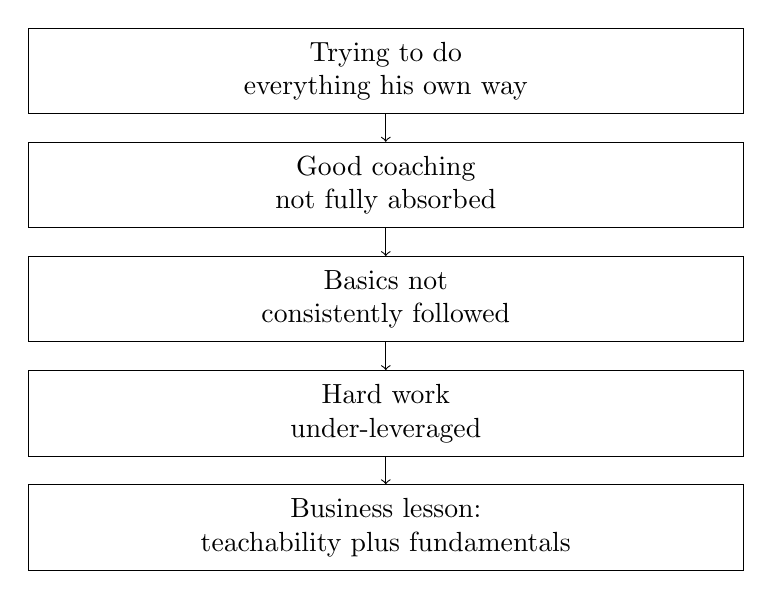
\begin{tikzpicture}[x=1cm,y=1cm]
\node[draw, align=center, text width=0.72\linewidth, inner sep=5pt] (a) at (0,0) {Trying to do\\everything his own way};
\node[draw, align=center, text width=0.72\linewidth, inner sep=5pt] (b) at (0,-1.45) {Good coaching\\not fully absorbed};
\node[draw, align=center, text width=0.72\linewidth, inner sep=5pt] (c) at (0,-2.90) {Basics not\\consistently followed};
\node[draw, align=center, text width=0.72\linewidth, inner sep=5pt] (d) at (0,-4.35) {Hard work\\under-leveraged};
\node[draw, align=center, text width=0.72\linewidth, inner sep=5pt] (e) at (0,-5.80) {Business lesson:\\teachability plus fundamentals};
\draw[->] (a) -- (b);
\draw[->] (b) -- (c);
\draw[->] (c) -- (d);
\draw[->] (d) -- (e);
\end{tikzpicture}
\caption{A transcript-backed reconstruction of the spoken mechanism. The lesson is not that effort is unimportant, but that effort compounds only when it is joined to coaching, basics, and judgment.}
\end{figure}

The figure should be read as an interpretive aid, not as a visual copied from a board. It preserves the order of the spoken answer: first self-directed execution, then incomplete absorption of coaching, then a failure to stay with basics, and finally the underuse of hard work.

\section{From Football Mistake to Business Judgment}

The business lesson should be stated with care because the excerpt ends at the diagnosis. We should not overbuild the claim. Still, the mechanism is clear enough to matter. A business owner can be energetic and still be weak where the work requires instruction. Drive is valuable, but drive can also protect a person from correction.

The football story therefore belongs in the broader entrepreneurship book under judgment, operations, and resilience. It is about judgment because the speaker had to learn that his own preferred way was not automatically the best way. It is about operations because basics are the repeatable parts of performance. It is about resilience because the useful lesson came from inspecting a mistake rather than polishing a success.

The narrow claim is stronger than a broad slogan. The lesson is not to obey every adviser or abandon independent judgment. The lesson is that when capable teachers are present, and when fundamentals are known, refusing to submit one's work to those fundamentals can waste even sincere effort.

\section{Summary}

The interview begins with the expected bridge from football to business: teamwork and adversity. It then turns toward the real lesson, which came from mistakes. As a quarterback at Long Beach City College, working with Brad Peabody and Ryan Flynn, the speaker had strong coaching available, but he kept trying to do things his own way.

The durable point is that hard work is not self-justifying. In business, as in sport, effort has to be joined to basics, instruction, and judgment. Otherwise a person can work intensely and still leave much of his ability unused.